\cajota{Participación en los Consejos de Desarrollo por sexo, según cargo }{\\[-0.7cm]La tabla muestra el número de mujeres y el número de hombres participando por consejo de desarrollo (para ver dicha desagregación por cargo, referirse a la Tabla 1 del apéndice A) de  2018 a 2022. Para el Consejo Nacional de Desarrollo Urbano y Rural, el año con el mayor número de mujeres fue 2020 y 2022 con 19 mujeres respectivamente. En los Consejos Regionales, Jutipa contó con el menor número de mujeres de todas  las regiones en los años reportados. Finalmente, en los Consejos Deparamentales, el menor número de mujeres participando en algún consejo en todos los años, se reportó en 2022 en San Marcos con 7 mujeres. }{Participación en los Consejos de Desarrollo por sexo, según cargo (número de personas)}{República de Guatemala, Instituto Nacional de Estadística}{\\[-1.7cm]\begin{tabular}[t]{cp{1cm}p{0.5cm}p{0.5cm}p{0.5cm}}
	\toprule
	\textbf{Tipo de delito} & \textbf{0-4} & \textbf{5-9} & \textbf{10-14} & \textbf{15-19}\\
	\midrule
	\cellcolor[HTML]{B6B3FF}{Violencia psicológica} & \cellcolor[HTML]{B6B3FF}{15} & \cellcolor[HTML]{B6B3FF}{5} & \cellcolor[HTML]{B6B3FF}{38} & \cellcolor[HTML]{B6B3FF}{770}\\
	Violencia física & 5 & 5 & 35 & 571 \\
	\cellcolor[HTML]{B6B3FF}{Violencia física y psicológica} & \cellcolor[HTML]{B6B3FF}{7} & \cellcolor[HTML]{B6B3FF}{NA} & \cellcolor[HTML]{B6B3FF}{28} & \cellcolor[HTML]{B6B3FF}{591}\\
	Violencia contra la mujer & 1 & 1 & 14 & 305 \\
	\cellcolor[HTML]{B6B3FF}{Violencia psicológica y económica} & \cellcolor[HTML]{B6B3FF}{NA} & \cellcolor[HTML]{B6B3FF}{NA} & \cellcolor[HTML]{B6B3FF}{NA} & \cellcolor[HTML]{B6B3FF}{24} \\
	Violencia física, psicológica y económica & 2 & NA & 1 & 24 \\
	\bottomrule
\end{tabular}
\\[1cm]
\begin{tabular}[t]{cp{1cm}p{0.5cm}p{0.5cm}p{0.5cm}}
	\toprule
	\textbf{Tipo de delito} & \textbf{0-4} & \textbf{5-9} & \textbf{10-14} & \textbf{15-19}\\
	\midrule
	\cellcolor[HTML]{B6B3FF}{Violencia psicológica} & \cellcolor[HTML]{B6B3FF}{15} & \cellcolor[HTML]{B6B3FF}{5} & \cellcolor[HTML]{B6B3FF}{38} & \cellcolor[HTML]{B6B3FF}{770}\\
	Violencia física & 5 & 5 & 35 & 571 \\
	\cellcolor[HTML]{B6B3FF}{Violencia física y psicológica} & \cellcolor[HTML]{B6B3FF}{7} & \cellcolor[HTML]{B6B3FF}{NA} & \cellcolor[HTML]{B6B3FF}{28} & \cellcolor[HTML]{B6B3FF}{591}\\
	Violencia contra la mujer & 1 & 1 & 14 & 305 \\
	\cellcolor[HTML]{B6B3FF}{Violencia psicológica y económica} & \cellcolor[HTML]{B6B3FF}{NA} & \cellcolor[HTML]{B6B3FF}{NA} & \cellcolor[HTML]{B6B3FF}{NA} & \cellcolor[HTML]{B6B3FF}{24} \\
	Violencia física, psicológica y económica & 2 & NA & 1 & 24 \\
	\bottomrule
\end{tabular}}{Secretaría General de Planificación -SEGEPLAN-, 2023}{}

\cajita{Personas electas para el Organismo Legislativo por sexo }{Según los reportes del Consejo de la Carrera Judicial del Organismo Judicial guatemalteco, para 2012, de las 154 diputaciones electas, 18 mujeres fueron electas. En 2016, esta cifra ascendió a 24 mujeres electas de 159 diputancias. Finalmente, en 2020 de las 156 diputaciones 32 de las personas electas fueron mujeres. }{Personas electas para el Organismo Legislativo por sexo (número de personas)}{República de Guatemala, Instituto Nacional de Estadística}{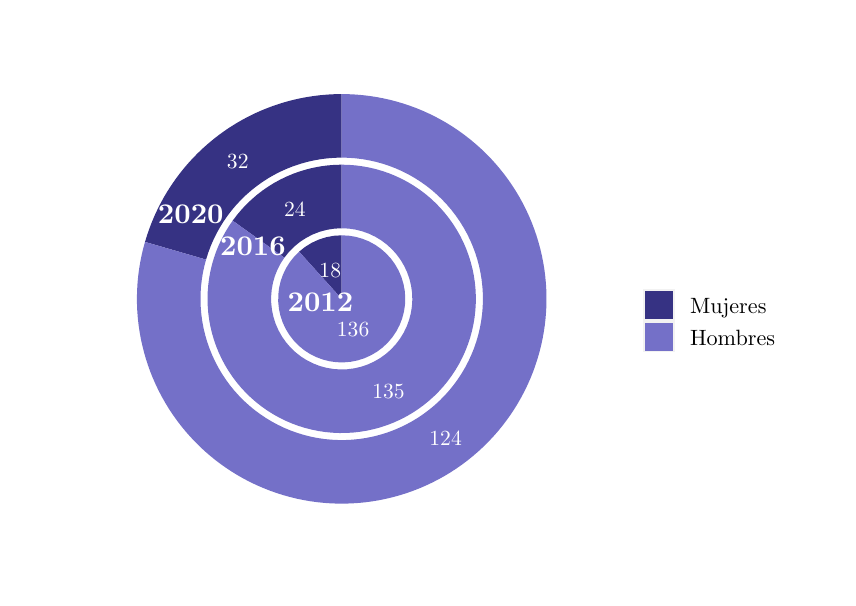
\begin{tikzpicture}[x=1pt,y=1pt]% Created by tikzDevice version 0.12.4 on 2023-05-24 15:32:14
% !TEX encoding = UTF-8 Unicode
\definecolor{fillColor}{RGB}{255,255,255}
\path[use as bounding box,fill=fillColor,fill opacity=0.00] (0,0) rectangle (289.08,198.74);
\begin{scope}
\path[clip] (  0.00,  0.00) rectangle (289.08,198.74);
\definecolor{drawColor}{RGB}{255,255,255}
\definecolor{fillColor}{RGB}{255,255,255}

\path[draw=drawColor,line width= 0.6pt,line join=round,line cap=round,fill=fillColor] ( 12.73,  0.00) rectangle (276.35,198.74);
\end{scope}
\begin{scope}
\path[clip] (  0.00,  0.00) rectangle (289.08,198.74);
\definecolor{fillColor}{RGB}{54,50,131}

\path[fill=fillColor] (113.47,100.75) --
	(113.47,103.30) --
	(113.47,105.85) --
	(113.47,108.40) --
	(113.47,110.95) --
	(113.47,113.50) --
	(113.47,116.06) --
	(113.47,118.61) --
	(113.47,121.16) --
	(113.47,123.71) --
	(110.67,123.54) --
	(107.91,123.03) --
	(105.23,122.18) --
	(102.67,121.01) --
	(100.28,119.54) --
	( 98.08,117.79) --
	( 99.79,115.90) --
	(101.50,114.00) --
	(103.21,112.11) --
	(104.92,110.22) --
	(106.63,108.32) --
	(108.34,106.43) --
	(110.05,104.53) --
	(111.76,102.64) --
	(113.47,100.75) --
	(113.47,100.75) --
	cycle;
\definecolor{fillColor}{RGB}{116,112,200}

\path[fill=fillColor] (113.47,100.75) --
	(111.76,102.64) --
	(110.05,104.53) --
	(108.34,106.43) --
	(106.63,108.32) --
	(104.92,110.22) --
	(103.21,112.11) --
	(101.50,114.00) --
	( 99.79,115.90) --
	( 98.08,117.79) --
	( 96.29,115.98) --
	( 94.71,113.99) --
	( 93.36,111.83) --
	( 92.26,109.53) --
	( 91.41,107.13) --
	( 90.84,104.64) --
	( 90.55,102.11) --
	( 90.54, 99.57) --
	( 90.81, 97.03) --
	( 91.36, 94.55) --
	( 92.18, 92.14) --
	( 93.27, 89.83) --
	( 94.60, 87.66) --
	( 96.17, 85.65) --
	( 97.95, 83.83) --
	( 99.91, 82.21) --
	(102.05, 80.82) --
	(104.33, 79.68) --
	(106.72, 78.80) --
	(109.19, 78.18) --
	(111.71, 77.85) --
	(114.26, 77.80) --
	(116.80, 78.02) --
	(119.29, 78.53) --
	(121.72, 79.31) --
	(124.04, 80.36) --
	(126.23, 81.65) --
	(128.27, 83.18) --
	(130.12, 84.93) --
	(131.77, 86.87) --
	(133.20, 88.98) --
	(134.38, 91.24) --
	(135.30, 93.61) --
	(135.96, 96.08) --
	(136.34, 98.59) --
	(136.43,101.14) --
	(136.25,103.68) --
	(135.78,106.18) --
	(135.05,108.62) --
	(134.04,110.96) --
	(132.78,113.18) --
	(131.29,115.24) --
	(129.57,117.12) --
	(127.66,118.81) --
	(125.57,120.27) --
	(123.34,121.49) --
	(120.98,122.45) --
	(118.53,123.15) --
	(116.02,123.57) --
	(113.47,123.71) --
	(113.47,121.16) --
	(113.47,118.61) --
	(113.47,116.06) --
	(113.47,113.50) --
	(113.47,110.95) --
	(113.47,108.40) --
	(113.47,105.85) --
	(113.47,103.30) --
	(113.47,100.75) --
	(113.47,100.75) --
	cycle;
\definecolor{fillColor}{RGB}{54,50,131}

\path[fill=fillColor] (113.47,126.26) --
	(113.47,128.81) --
	(113.47,131.37) --
	(113.47,133.92) --
	(113.47,136.47) --
	(113.47,139.02) --
	(113.47,141.57) --
	(113.47,144.12) --
	(113.47,146.68) --
	(113.47,149.23) --
	(110.92,149.16) --
	(108.37,148.96) --
	(105.84,148.62) --
	(103.33,148.15) --
	(100.85,147.55) --
	( 98.40,146.82) --
	( 96.00,145.97) --
	( 93.64,144.98) --
	( 91.34,143.88) --
	( 89.09,142.65) --
	( 86.92,141.31) --
	( 84.82,139.86) --
	( 82.80,138.29) --
	( 80.87,136.62) --
	( 79.02,134.86) --
	( 77.27,133.00) --
	( 75.63,131.04) --
	( 74.08,129.01) --
	( 76.16,127.52) --
	( 78.23,126.03) --
	( 80.30,124.55) --
	( 82.38,123.06) --
	( 84.45,121.57) --
	( 86.52,120.08) --
	( 88.60,118.60) --
	( 90.67,117.11) --
	( 92.74,115.62) --
	( 94.42,117.72) --
	( 96.31,119.63) --
	( 98.39,121.33) --
	(100.64,122.80) --
	(103.03,124.03) --
	(105.54,125.00) --
	(108.14,125.70) --
	(110.79,126.12) --
	(113.47,126.26) --
	cycle;
\definecolor{fillColor}{RGB}{116,112,200}

\path[fill=fillColor] ( 92.74,115.62) --
	( 90.67,117.11) --
	( 88.60,118.60) --
	( 86.52,120.08) --
	( 84.45,121.57) --
	( 82.38,123.06) --
	( 80.30,124.55) --
	( 78.23,126.03) --
	( 76.16,127.52) --
	( 74.08,129.01) --
	( 72.67,126.93) --
	( 71.37,124.79) --
	( 70.18,122.57) --
	( 69.11,120.30) --
	( 68.16,117.98) --
	( 67.33,115.61) --
	( 66.62,113.20) --
	( 66.04,110.76) --
	( 65.58,108.29) --
	( 65.26,105.80) --
	( 65.06,103.30) --
	( 64.99,100.79) --
	( 65.06, 98.28) --
	( 65.25, 95.77) --
	( 65.57, 93.28) --
	( 66.02, 90.81) --
	( 66.60, 88.37) --
	( 67.30, 85.96) --
	( 68.13, 83.59) --
	( 69.08, 81.27) --
	( 70.15, 78.99) --
	( 71.33, 76.78) --
	( 72.63, 74.63) --
	( 74.03, 72.55) --
	( 75.55, 70.55) --
	( 77.16, 68.62) --
	( 78.87, 66.79) --
	( 80.68, 65.04) --
	( 82.57, 63.39) --
	( 84.55, 61.84) --
	( 86.60, 60.40) --
	( 88.72, 59.06) --
	( 90.91, 57.83) --
	( 93.17, 56.72) --
	( 95.47, 55.73) --
	( 97.83, 54.86) --
	(100.22, 54.11) --
	(102.66, 53.49) --
	(105.12, 52.99) --
	(107.60, 52.62) --
	(110.10, 52.38) --
	(112.61, 52.27) --
	(115.12, 52.29) --
	(117.63, 52.44) --
	(120.12, 52.72) --
	(122.60, 53.13) --
	(125.05, 53.67) --
	(127.47, 54.33) --
	(129.86, 55.12) --
	(132.20, 56.03) --
	(134.49, 57.06) --
	(136.72, 58.20) --
	(138.89, 59.46) --
	(141.00, 60.83) --
	(143.02, 62.31) --
	(144.97, 63.89) --
	(146.84, 65.57) --
	(148.62, 67.35) --
	(150.30, 69.21) --
	(151.88, 71.16) --
	(153.36, 73.19) --
	(154.73, 75.29) --
	(156.00, 77.46) --
	(157.15, 79.70) --
	(158.18, 81.98) --
	(159.09, 84.32) --
	(159.88, 86.71) --
	(160.54, 89.13) --
	(161.08, 91.58) --
	(161.49, 94.06) --
	(161.77, 96.55) --
	(161.92, 99.06) --
	(161.95,101.57) --
	(161.84,104.08) --
	(161.60,106.58) --
	(161.24,109.06) --
	(160.74,111.52) --
	(160.12,113.96) --
	(159.37,116.35) --
	(158.50,118.71) --
	(157.51,121.02) --
	(156.41,123.27) --
	(155.18,125.46) --
	(153.85,127.59) --
	(152.40,129.64) --
	(150.85,131.62) --
	(149.21,133.51) --
	(147.46,135.32) --
	(145.63,137.03) --
	(143.71,138.65) --
	(141.70,140.16) --
	(139.62,141.57) --
	(137.48,142.87) --
	(135.26,144.05) --
	(132.99,145.12) --
	(130.67,146.08) --
	(128.30,146.90) --
	(125.89,147.61) --
	(123.45,148.19) --
	(120.98,148.64) --
	(118.49,148.97) --
	(115.98,149.16) --
	(113.47,149.23) --
	(113.47,146.68) --
	(113.47,144.12) --
	(113.47,141.57) --
	(113.47,139.02) --
	(113.47,136.47) --
	(113.47,133.92) --
	(113.47,131.37) --
	(113.47,128.81) --
	(113.47,126.26) --
	(115.99,126.14) --
	(118.48,125.77) --
	(120.93,125.15) --
	(123.30,124.30) --
	(125.57,123.21) --
	(127.73,121.91) --
	(129.75,120.40) --
	(131.61,118.70) --
	(133.29,116.82) --
	(134.78,114.79) --
	(136.06,112.62) --
	(137.12,110.34) --
	(137.95,107.96) --
	(138.54,105.51) --
	(138.89,103.01) --
	(138.99,100.49) --
	(138.84, 97.98) --
	(138.44, 95.49) --
	(137.80, 93.05) --
	(136.92, 90.69) --
	(135.82, 88.43) --
	(134.49, 86.28) --
	(132.97, 84.28) --
	(131.25, 82.44) --
	(129.35, 80.77) --
	(127.31, 79.31) --
	(125.12, 78.05) --
	(122.83, 77.01) --
	(120.44, 76.20) --
	(117.99, 75.63) --
	(115.49, 75.31) --
	(112.97, 75.24) --
	(110.46, 75.41) --
	(107.97, 75.83) --
	(105.54, 76.49) --
	(103.19, 77.40) --
	(100.93, 78.52) --
	( 98.80, 79.87) --
	( 96.82, 81.42) --
	( 94.99, 83.15) --
	( 93.35, 85.06) --
	( 91.90, 87.13) --
	( 90.66, 89.32) --
	( 89.64, 91.63) --
	( 88.86, 94.02) --
	( 88.32, 96.48) --
	( 88.02, 98.98) --
	( 87.97,101.50) --
	( 88.17,104.01) --
	( 88.61,106.49) --
	( 89.30,108.92) --
	( 90.23,111.26) --
	( 91.38,113.50) --
	( 92.74,115.62) --
	cycle;
\definecolor{fillColor}{RGB}{54,50,131}

\path[fill=fillColor] (113.47,151.78) --
	(113.47,154.33) --
	(113.47,156.88) --
	(113.47,159.43) --
	(113.47,161.99) --
	(113.47,164.54) --
	(113.47,167.09) --
	(113.47,169.64) --
	(113.47,172.19) --
	(113.47,174.74) --
	(110.96,174.70) --
	(108.46,174.57) --
	(105.96,174.36) --
	(103.47,174.06) --
	(100.98,173.68) --
	( 98.52,173.22) --
	( 96.07,172.67) --
	( 93.64,172.04) --
	( 91.23,171.32) --
	( 88.85,170.53) --
	( 86.50,169.65) --
	( 84.18,168.70) --
	( 81.89,167.67) --
	( 79.64,166.56) --
	( 77.43,165.37) --
	( 75.26,164.11) --
	( 73.13,162.78) --
	( 71.05,161.38) --
	( 69.02,159.90) --
	( 67.04,158.36) --
	( 65.11,156.75) --
	( 63.24,155.08) --
	( 61.43,153.35) --
	( 59.67,151.55) --
	( 57.98,149.70) --
	( 56.35,147.79) --
	( 54.79,145.82) --
	( 53.30,143.81) --
	( 51.87,141.74) --
	( 50.52,139.63) --
	( 49.23,137.47) --
	( 48.03,135.27) --
	( 46.89,133.03) --
	( 45.84,130.76) --
	( 44.86,128.45) --
	( 43.96,126.10) --
	( 43.14,123.73) --
	( 42.40,121.33) --
	( 44.85,120.62) --
	( 47.30,119.91) --
	( 49.75,119.20) --
	( 52.20,118.49) --
	( 54.65,117.78) --
	( 57.10,117.07) --
	( 59.55,116.36) --
	( 62.00,115.65) --
	( 64.46,114.94) --
	( 65.22,117.36) --
	( 66.10,119.73) --
	( 67.10,122.05) --
	( 68.21,124.32) --
	( 69.44,126.54) --
	( 70.77,128.69) --
	( 72.21,130.77) --
	( 73.74,132.78) --
	( 75.38,134.71) --
	( 77.11,136.55) --
	( 78.93,138.31) --
	( 80.83,139.97) --
	( 82.82,141.54) --
	( 84.88,143.01) --
	( 87.00,144.38) --
	( 89.20,145.64) --
	( 91.45,146.78) --
	( 93.76,147.82) --
	( 96.12,148.74) --
	( 98.52,149.54) --
	(100.95,150.22) --
	(103.42,150.78) --
	(105.91,151.22) --
	(108.42,151.53) --
	(110.94,151.72) --
	(113.47,151.78) --
	cycle;
\definecolor{fillColor}{RGB}{116,112,200}

\path[fill=fillColor] ( 64.46,114.94) --
	( 62.00,115.65) --
	( 59.55,116.36) --
	( 57.10,117.07) --
	( 54.65,117.78) --
	( 52.20,118.49) --
	( 49.75,119.20) --
	( 47.30,119.91) --
	( 44.85,120.62) --
	( 42.40,121.33) --
	( 41.74,118.91) --
	( 41.16,116.46) --
	( 40.67,113.99) --
	( 40.26,111.51) --
	( 39.94,109.02) --
	( 39.70,106.52) --
	( 39.55,104.01) --
	( 39.48,101.50) --
	( 39.50, 98.98) --
	( 39.60, 96.47) --
	( 39.79, 93.96) --
	( 40.06, 91.46) --
	( 40.42, 88.98) --
	( 40.86, 86.50) --
	( 41.39, 84.04) --
	( 42.00, 81.60) --
	( 42.69, 79.19) --
	( 43.46, 76.80) --
	( 44.31, 74.43) --
	( 45.25, 72.10) --
	( 46.26, 69.80) --
	( 47.35, 67.53) --
	( 48.52, 65.30) --
	( 49.76, 63.12) --
	( 51.07, 60.97) --
	( 52.46, 58.88) --
	( 53.92, 56.83) --
	( 55.44, 54.83) --
	( 57.04, 52.89) --
	( 58.70, 51.00) --
	( 60.42, 49.17) --
	( 62.20, 47.39) --
	( 64.04, 45.68) --
	( 65.94, 44.04) --
	( 67.89, 42.45) --
	( 69.90, 40.94) --
	( 71.96, 39.49) --
	( 74.06, 38.12) --
	( 76.21, 36.82) --
	( 78.40, 35.59) --
	( 80.64, 34.43) --
	( 82.91, 33.36) --
	( 85.22, 32.36) --
	( 87.56, 31.44) --
	( 89.93, 30.60) --
	( 92.32, 29.84) --
	( 94.74, 29.16) --
	( 97.19, 28.56) --
	( 99.65, 28.05) --
	(102.12, 27.62) --
	(104.61, 27.28) --
	(107.12, 27.02) --
	(109.62, 26.85) --
	(112.14, 26.76) --
	(114.65, 26.76) --
	(117.16, 26.84) --
	(119.67, 27.01) --
	(122.17, 27.26) --
	(124.66, 27.60) --
	(127.14, 28.02) --
	(129.60, 28.53) --
	(132.05, 29.12) --
	(134.47, 29.79) --
	(136.87, 30.54) --
	(139.24, 31.38) --
	(141.58, 32.29) --
	(143.89, 33.29) --
	(146.16, 34.36) --
	(148.40, 35.51) --
	(150.59, 36.73) --
	(152.75, 38.03) --
	(154.86, 39.40) --
	(156.92, 40.84) --
	(158.93, 42.35) --
	(160.88, 43.93) --
	(162.78, 45.57) --
	(164.63, 47.28) --
	(166.42, 49.05) --
	(168.14, 50.88) --
	(169.81, 52.76) --
	(171.40, 54.71) --
	(172.93, 56.70) --
	(174.39, 58.74) --
	(175.79, 60.84) --
	(177.11, 62.98) --
	(178.35, 65.16) --
	(179.52, 67.39) --
	(180.62, 69.65) --
	(181.64, 71.95) --
	(182.58, 74.28) --
	(183.43, 76.64) --
	(184.21, 79.03) --
	(184.91, 81.45) --
	(185.52, 83.89) --
	(186.06, 86.34) --
	(186.50, 88.82) --
	(186.87, 91.30) --
	(187.14, 93.80) --
	(187.34, 96.31) --
	(187.45, 98.82) --
	(187.47,101.33) --
	(187.41,103.85) --
	(187.26,106.36) --
	(187.02,108.86) --
	(186.71,111.35) --
	(186.30,113.84) --
	(185.82,116.30) --
	(185.25,118.75) --
	(184.59,121.18) --
	(183.86,123.58) --
	(183.04,125.96) --
	(182.15,128.31) --
	(181.17,130.62) --
	(180.12,132.91) --
	(178.99,135.15) --
	(177.78,137.36) --
	(176.50,139.52) --
	(175.14,141.64) --
	(173.72,143.71) --
	(172.23,145.73) --
	(170.66,147.70) --
	(169.04,149.62) --
	(167.34,151.48) --
	(165.59,153.28) --
	(163.77,155.02) --
	(161.90,156.69) --
	(159.97,158.31) --
	(157.99,159.85) --
	(155.96,161.33) --
	(153.88,162.74) --
	(151.75,164.08) --
	(149.57,165.34) --
	(147.36,166.53) --
	(145.10,167.64) --
	(142.81,168.68) --
	(140.49,169.64) --
	(138.13,170.51) --
	(135.75,171.31) --
	(133.34,172.03) --
	(130.91,172.66) --
	(128.45,173.21) --
	(125.98,173.68) --
	(123.50,174.06) --
	(121.00,174.36) --
	(118.50,174.57) --
	(115.99,174.70) --
	(113.47,174.74) --
	(113.47,172.19) --
	(113.47,169.64) --
	(113.47,167.09) --
	(113.47,164.54) --
	(113.47,161.99) --
	(113.47,159.43) --
	(113.47,156.88) --
	(113.47,154.33) --
	(113.47,151.78) --
	(116.00,151.72) --
	(118.51,151.53) --
	(121.02,151.22) --
	(123.50,150.78) --
	(125.96,150.23) --
	(128.39,149.55) --
	(130.79,148.75) --
	(133.14,147.84) --
	(135.44,146.81) --
	(137.69,145.67) --
	(139.88,144.41) --
	(142.01,143.05) --
	(144.07,141.59) --
	(146.05,140.03) --
	(147.95,138.37) --
	(149.77,136.62) --
	(151.50,134.78) --
	(153.13,132.86) --
	(154.67,130.86) --
	(156.11,128.79) --
	(157.44,126.65) --
	(158.67,124.44) --
	(159.79,122.18) --
	(160.79,119.87) --
	(161.68,117.50) --
	(162.45,115.10) --
	(163.10,112.66) --
	(163.62,110.20) --
	(164.03,107.70) --
	(164.31,105.20) --
	(164.47,102.68) --
	(164.50,100.16) --
	(164.41, 97.63) --
	(164.19, 95.12) --
	(163.85, 92.62) --
	(163.39, 90.14) --
	(162.81, 87.69) --
	(162.10, 85.26) --
	(161.28, 82.88) --
	(160.33, 80.54) --
	(159.28, 78.25) --
	(158.11, 76.01) --
	(156.83, 73.83) --
	(155.45, 71.72) --
	(153.96, 69.68) --
	(152.38, 67.72) --
	(150.70, 65.84) --
	(148.93, 64.04) --
	(147.07, 62.33) --
	(145.13, 60.72) --
	(143.11, 59.20) --
	(141.02, 57.79) --
	(138.87, 56.48) --
	(136.65, 55.28) --
	(134.37, 54.19) --
	(132.04, 53.21) --
	(129.67, 52.35) --
	(127.26, 51.61) --
	(124.82, 50.99) --
	(122.34, 50.49) --
	(119.85, 50.11) --
	(117.34, 49.86) --
	(114.82, 49.73) --
	(112.29, 49.73) --
	(109.77, 49.85) --
	(107.26, 50.09) --
	(104.77, 50.46) --
	(102.29, 50.95) --
	( 99.84, 51.57) --
	( 97.43, 52.30) --
	( 95.05, 53.15) --
	( 92.72, 54.12) --
	( 90.44, 55.21) --
	( 88.22, 56.40) --
	( 86.06, 57.70) --
	( 83.97, 59.11) --
	( 81.94, 60.62) --
	( 80.00, 62.23) --
	( 78.14, 63.93) --
	( 76.36, 65.72) --
	( 74.67, 67.60) --
	( 73.08, 69.55) --
	( 71.59, 71.59) --
	( 70.20, 73.70) --
	( 68.92, 75.87) --
	( 67.74, 78.10) --
	( 66.68, 80.39) --
	( 65.73, 82.73) --
	( 64.90, 85.11) --
	( 64.18, 87.53) --
	( 63.59, 89.98) --
	( 63.12, 92.46) --
	( 62.77, 94.96) --
	( 62.55, 97.47) --
	( 62.45, 99.99) --
	( 62.47,102.52) --
	( 62.62,105.04) --
	( 62.90,107.54) --
	( 63.29,110.04) --
	( 63.81,112.50) --
	( 64.46,114.94) --
	cycle;
\definecolor{drawColor}{RGB}{255,255,255}

\node[text=drawColor,anchor=base,inner sep=0pt, outer sep=0pt, scale=  0.78] at (109.35,108.43) {18};

\node[text=drawColor,anchor=base,inner sep=0pt, outer sep=0pt, scale=  0.78] at (117.60, 87.00) {136};

\node[text=drawColor,anchor=base,inner sep=0pt, outer sep=0pt, scale=  0.78] at ( 96.58,130.63) {24};

\node[text=drawColor,anchor=base,inner sep=0pt, outer sep=0pt, scale=  0.78] at (130.37, 64.80) {135};

\node[text=drawColor,anchor=base,inner sep=0pt, outer sep=0pt, scale=  0.78] at ( 75.92,147.69) {32};

\node[text=drawColor,anchor=base,inner sep=0pt, outer sep=0pt, scale=  0.78] at (151.03, 47.74) {124};

\node[text=drawColor,anchor=base,inner sep=0pt, outer sep=0pt, scale=  1.03] at (105.78,96.22) {\bfseries 2012};

\node[text=drawColor,anchor=base,inner sep=0pt, outer sep=0pt, scale=  1.03] at ( 81.41,116.27) {\bfseries 2016};

\node[text=drawColor,anchor=base,inner sep=0pt, outer sep=0pt, scale=  1.03] at ( 58.93,128.09) {\bfseries 2020};
\end{scope}
\begin{scope}
\path[clip] (  0.00,  0.00) rectangle (289.08,198.74);
\definecolor{fillColor}{RGB}{255,255,255}

\path[fill=fillColor] (216.97, 75.89) rectangle (270.85,125.60);
\end{scope}
\begin{scope}
\path[clip] (  0.00,  0.00) rectangle (289.08,198.74);
\definecolor{fillColor}{gray}{0.95}

\path[fill=fillColor] (222.47, 92.77) rectangle (233.85,104.15);
\end{scope}
\begin{scope}
\path[clip] (  0.00,  0.00) rectangle (289.08,198.74);
\definecolor{fillColor}{RGB}{54,50,131}

\path[fill=fillColor] (223.13, 93.44) rectangle (233.19,103.49);
\end{scope}
\begin{scope}
\path[clip] (  0.00,  0.00) rectangle (289.08,198.74);
\definecolor{fillColor}{gray}{0.95}

\path[fill=fillColor] (222.47, 81.39) rectangle (233.85, 92.77);
\end{scope}
\begin{scope}
\path[clip] (  0.00,  0.00) rectangle (289.08,198.74);
\definecolor{fillColor}{RGB}{116,112,200}

\path[fill=fillColor] (223.13, 82.05) rectangle (233.19, 92.11);
\end{scope}
\begin{scope}
\path[clip] (  0.00,  0.00) rectangle (289.08,198.74);
\definecolor{drawColor}{RGB}{0,0,0}

\node[text=drawColor,anchor=base west,inner sep=0pt, outer sep=0pt, scale=  0.80] at (239.35, 95.34) {Mujeres};
\end{scope}
\begin{scope}
\path[clip] (  0.00,  0.00) rectangle (289.08,198.74);
\definecolor{drawColor}{RGB}{0,0,0}

\node[text=drawColor,anchor=base west,inner sep=0pt, outer sep=0pt, scale=  0.80] at (239.35, 83.96) {Hombres};
\end{scope}
\end{tikzpicture}}{Unidad de Acceso a la Informacion - Congreso de la República de Guatemala 2023}{}

\cajita{Mujeres magistradas en el Organismo Judicial}{Hola :)}{Mujeres magistradas en el Organismo Judicial (número de mujeres)}{República de Guatemala, Instituto Nacional de Estadística}{\begin{tikzpicture}[x=1pt,y=1pt]Hola :)
\end{tikzpicture}}{Datos públicos Organismo Legislatico 2023}{}

\cajita{Mujeres electas para alcaldías}{Según datos públicos del Informe 2019 del Tribunal Supremo Electoral, para 2020, de las 340 alcaldías en Guatemala, 8 fueron electas para ser ocupadas por mujeres. }{Mujeres electas para alcaldías (número de mujeres)}{República de Guatemala, Instituto Nacional de Estadística}{\begin{tikzpicture}[x=1pt,y=1pt]% Created by tikzDevice version 0.12.4 on 2023-05-25 10:59:49
% !TEX encoding = UTF-8 Unicode
\definecolor{fillColor}{RGB}{255,255,255}
\path[use as bounding box,fill=fillColor,fill opacity=0.00] (0,0) rectangle (289.08,198.74);
\begin{scope}
\path[clip] ( 31.85,  0.00) rectangle (257.23,198.74);

\path[] ( 31.85,  0.00) rectangle (257.23,198.74);
\end{scope}
\begin{scope}
\path[clip] (  0.00,  0.00) rectangle (289.08,198.74);
\definecolor{drawColor}{RGB}{255,255,255}
\definecolor{fillColor}{RGB}{54,50,131}

\path[draw=drawColor,line width= 0.6pt,fill=color2] ( 98.38,140.98) --
	( 97.98,143.68) --
	( 97.57,146.38) --
	( 97.17,149.08) --
	( 96.77,151.78) --
	( 96.37,154.48) --
	( 95.96,157.18) --
	( 95.56,159.88) --
	( 95.16,162.59) --
	( 94.76,165.29) --
	( 94.36,167.99) --
	( 93.95,170.69) --
	( 93.55,173.39) --
	( 93.15,176.09) --
	( 92.75,178.79) --
	( 90.19,178.37) --
	( 87.65,177.86) --
	( 85.13,177.26) --
	( 82.63,176.58) --
	( 80.15,175.81) --
	( 77.70,174.96) --
	( 75.28,174.03) --
	( 72.90,173.01) --
	( 70.55,171.92) --
	( 68.24,170.74) --
	( 65.97,169.49) --
	( 63.74,168.16) --
	( 61.56,166.76) --
	( 59.43,165.29) --
	( 57.35,163.74) --
	( 55.33,162.13) --
	( 53.36,160.44) --
	( 51.44,158.69) --
	( 49.59,156.88) --
	( 47.80,155.00) --
	( 46.08,153.07) --
	( 44.42,151.08) --
	( 42.83,149.03) --
	( 41.31,146.93) --
	( 39.86,144.78) --
	( 38.49,142.58) --
	( 37.19,140.34) --
	( 35.97,138.05) --
	( 34.83,135.73) --
	( 33.76,133.36) --
	( 32.78,130.97) --
	( 31.88,128.54) --
	( 31.06,126.08) --
	( 30.32,123.59) --
	( 29.67,121.08) --
	( 29.11,118.55) --
	( 28.63,116.01) --
	( 28.24,113.44) --
	( 27.93,110.87) --
	( 27.72,108.29) --
	( 27.59,105.70) --
	( 27.54,103.11) --
	( 27.59,100.52) --
	( 27.72, 97.93) --
	( 27.95, 95.34) --
	( 28.25, 92.77) --
	( 28.65, 90.21) --
	( 29.13, 87.66) --
	( 29.70, 85.13) --
	( 30.35, 82.63) --
	( 31.09, 80.14) --
	( 31.91, 77.68) --
	( 32.82, 75.26) --
	( 33.81, 72.86) --
	( 34.87, 70.50) --
	( 36.02, 68.17) --
	( 37.24, 65.89) --
	( 38.55, 63.65) --
	( 39.92, 61.45) --
	( 41.37, 59.30) --
	( 42.90, 57.21) --
	( 44.49, 55.16) --
	( 46.15, 53.17) --
	( 47.88, 51.24) --
	( 49.67, 49.37) --
	( 51.52, 47.56) --
	( 53.44, 45.81) --
	( 55.41, 44.13) --
	( 57.44, 42.51) --
	( 59.52, 40.97) --
	( 61.65, 39.50) --
	( 63.84, 38.10) --
	( 66.06, 36.78) --
	( 68.34, 35.53) --
	( 70.65, 34.36) --
	( 73.00, 33.27) --
	( 75.39, 32.26) --
	( 77.80, 31.33) --
	( 80.25, 30.48) --
	( 82.73, 29.72) --
	( 85.23, 29.04) --
	( 87.76, 28.44) --
	( 90.30, 27.94) --
	( 92.85, 27.51) --
	( 95.42, 27.18) --
	( 98.00, 26.93) --
	(100.59, 26.77) --
	(103.18, 26.70) --
	(105.77, 26.72) --
	(108.36, 26.82) --
	(110.95, 27.01) --
	(113.52, 27.29) --
	(116.09, 27.66) --
	(118.64, 28.11) --
	(121.18, 28.65) --
	(123.69, 29.27) --
	(126.19, 29.98) --
	(128.65, 30.78) --
	(131.09, 31.65) --
	(133.50, 32.61) --
	(135.87, 33.65) --
	(138.21, 34.77) --
	(140.51, 35.97) --
	(142.77, 37.25) --
	(144.98, 38.60) --
	(147.14, 40.02) --
	(149.26, 41.52) --
	(151.32, 43.09) --
	(153.33, 44.73) --
	(155.28, 46.43) --
	(157.17, 48.20) --
	(159.01, 50.04) --
	(160.77, 51.93) --
	(162.48, 53.88) --
	(164.11, 55.89) --
	(165.68, 57.96) --
	(167.18, 60.07) --
	(168.60, 62.24) --
	(169.95, 64.45) --
	(171.23, 66.71) --
	(172.42, 69.01) --
	(173.54, 71.35) --
	(174.58, 73.72) --
	(175.54, 76.13) --
	(176.41, 78.57) --
	(177.20, 81.04) --
	(177.91, 83.53) --
	(178.53, 86.05) --
	(179.07, 88.58) --
	(179.52, 91.13) --
	(179.89, 93.70) --
	(180.16, 96.28) --
	(180.35, 98.86) --
	(180.46,101.45) --
	(180.47,104.04) --
	(180.40,106.63) --
	(180.23,109.22) --
	(179.98,111.80) --
	(179.65,114.37) --
	(179.22,116.93) --
	(178.72,119.47) --
	(178.12,121.99) --
	(177.44,124.49) --
	(176.67,126.97) --
	(175.83,129.42) --
	(174.89,131.84) --
	(173.88,134.22) --
	(172.79,136.57) --
	(171.62,138.88) --
	(170.37,141.15) --
	(169.04,143.38) --
	(167.64,145.56) --
	(166.17,147.69) --
	(164.62,149.78) --
	(163.01,151.80) --
	(161.33,153.77) --
	(159.58,155.69) --
	(157.77,157.54) --
	(155.89,159.33) --
	(153.96,161.06) --
	(151.97,162.72) --
	(149.92,164.31) --
	(147.82,165.83) --
	(145.67,167.28) --
	(143.48,168.65) --
	(141.23,169.95) --
	(138.95,171.18) --
	(136.62,172.32) --
	(134.26,173.39) --
	(131.86,174.37) --
	(129.44,175.28) --
	(126.98,176.10) --
	(124.49,176.83) --
	(121.98,177.48) --
	(119.45,178.05) --
	(116.91,178.53) --
	(114.35,178.92) --
	(111.77,179.23) --
	(109.19,179.45) --
	(106.60,179.58) --
	(104.01,179.63) --
	(104.01,176.90) --
	(104.01,174.16) --
	(104.01,171.43) --
	(104.01,168.70) --
	(104.01,165.97) --
	(104.01,163.24) --
	(104.01,160.51) --
	(104.01,157.78) --
	(104.01,155.05) --
	(104.01,152.32) --
	(104.01,149.59) --
	(104.01,146.86) --
	(104.01,144.12) --
	(104.01,141.39) --
	(106.61,141.31) --
	(109.21,141.04) --
	(111.77,140.60) --
	(114.31,139.98) --
	(116.79,139.19) --
	(119.22,138.24) --
	(121.57,137.12) --
	(123.84,135.85) --
	(126.02,134.42) --
	(128.10,132.85) --
	(130.07,131.14) --
	(131.91,129.30) --
	(133.63,127.34) --
	(135.21,125.26) --
	(136.64,123.09) --
	(137.92,120.82) --
	(139.04,118.47) --
	(140.01,116.05) --
	(140.80,113.56) --
	(141.42,111.03) --
	(141.87,108.47) --
	(142.15,105.88) --
	(142.24,103.27) --
	(142.16,100.67) --
	(141.90, 98.07) --
	(141.47, 95.50) --
	(140.86, 92.97) --
	(140.08, 90.48) --
	(139.13, 88.06) --
	(138.02, 85.70) --
	(136.75, 83.42) --
	(135.33, 81.24) --
	(133.77, 79.16) --
	(132.06, 77.18) --
	(130.23, 75.33) --
	(128.27, 73.61) --
	(126.20, 72.03) --
	(124.03, 70.59) --
	(121.76, 69.30) --
	(119.42, 68.17) --
	(117.00, 67.20) --
	(114.52, 66.40) --
	(111.99, 65.77) --
	(109.42, 65.31) --
	(106.83, 65.03) --
	(104.23, 64.93) --
	(101.62, 65.00) --
	( 99.03, 65.25) --
	( 96.46, 65.68) --
	( 93.92, 66.28) --
	( 91.44, 67.06) --
	( 89.01, 68.00) --
	( 86.65, 69.10) --
	( 84.37, 70.36) --
	( 82.18, 71.78) --
	( 80.09, 73.34) --
	( 78.11, 75.03) --
	( 76.26, 76.86) --
	( 74.53, 78.82) --
	( 72.94, 80.88) --
	( 71.50, 83.05) --
	( 70.20, 85.31) --
	( 69.06, 87.65) --
	( 68.09, 90.07) --
	( 67.28, 92.55) --
	( 66.64, 95.07) --
	( 66.18, 97.64) --
	( 65.89,100.23) --
	( 65.78,102.83) --
	( 65.84,105.44) --
	( 66.09,108.03) --
	( 66.51,110.60) --
	( 67.10,113.14) --
	( 67.87,115.63) --
	( 68.80,118.06) --
	( 69.90,120.43) --
	( 71.15,122.71) --
	( 72.56,124.90) --
	( 74.12,127.00) --
	( 75.81,128.98) --
	( 77.63,130.84) --
	( 79.58,132.57) --
	( 81.64,134.17) --
	( 83.80,135.62) --
	( 86.06,136.92) --
	( 88.40,138.06) --
	( 90.82,139.05) --
	( 93.29,139.86) --
	( 95.81,140.51) --
	( 98.38,140.98) --
	cycle;
\definecolor{fillColor}{RGB}{116,112,200}

\path[draw=drawColor,line width= 0.6pt,fill=color3] (104.01,141.39) --
	(104.01,144.12) --
	(104.01,146.86) --
	(104.01,149.59) --
	(104.01,152.32) --
	(104.01,155.05) --
	(104.01,157.78) --
	(104.01,160.51) --
	(104.01,163.24) --
	(104.01,165.97) --
	(104.01,168.70) --
	(104.01,171.43) --
	(104.01,174.16) --
	(104.01,176.90) --
	(104.01,179.63) --
	(101.18,179.57) --
	( 98.36,179.42) --
	( 95.55,179.16) --
	( 92.75,178.79) --
	( 93.15,176.09) --
	( 93.55,173.39) --
	( 93.95,170.69) --
	( 94.36,167.99) --
	( 94.76,165.29) --
	( 95.16,162.59) --
	( 95.56,159.88) --
	( 95.96,157.18) --
	( 96.37,154.48) --
	( 96.77,151.78) --
	( 97.17,149.08) --
	( 97.57,146.38) --
	( 97.98,143.68) --
	( 98.38,140.98) --
	(101.19,141.29) --
	(104.01,141.39) --
	cycle;

\path[] (  8.43,  7.58) rectangle (199.59,198.74);

\path[] (104.01,103.16) --
	(110.36, 17.37);

\path[] (104.01,103.16) --
	( 97.66,188.95);

\path[] (104.01,103.16) --
	(189.80,109.51);

\path[] (104.01,103.16) --
	(110.36, 17.37);

\path[] (104.01,103.16) --
	( 18.22, 96.81);

\path[] (104.01,103.16) --
	( 97.66,188.95);

\path[] (104.01,103.16) --
	(104.01,103.16) --
	(104.01,103.16) --
	(104.01,103.16) --
	(104.01,103.16) --
	(104.01,103.16) --
	(104.01,103.16) --
	(104.01,103.16) --
	(104.01,103.16) --
	(104.01,103.16) --
	(104.01,103.16) --
	(104.01,103.16) --
	(104.01,103.16) --
	(104.01,103.16) --
	(104.01,103.16) --
	(104.01,103.16) --
	(104.01,103.16) --
	(104.01,103.16) --
	(104.01,103.16) --
	(104.01,103.16) --
	(104.01,103.16) --
	(104.01,103.16) --
	(104.01,103.16) --
	(104.01,103.16) --
	(104.01,103.16) --
	(104.01,103.16) --
	(104.01,103.16) --
	(104.01,103.16) --
	(104.01,103.16) --
	(104.01,103.16) --
	(104.01,103.16) --
	(104.01,103.16) --
	(104.01,103.16) --
	(104.01,103.16) --
	(104.01,103.16) --
	(104.01,103.16) --
	(104.01,103.16) --
	(104.01,103.16) --
	(104.01,103.16) --
	(104.01,103.16) --
	(104.01,103.16) --
	(104.01,103.16) --
	(104.01,103.16) --
	(104.01,103.16) --
	(104.01,103.16) --
	(104.01,103.16) --
	(104.01,103.16) --
	(104.01,103.16) --
	(104.01,103.16) --
	(104.01,103.16) --
	(104.01,103.16) --
	(104.01,103.16) --
	(104.01,103.16) --
	(104.01,103.16) --
	(104.01,103.16) --
	(104.01,103.16) --
	(104.01,103.16) --
	(104.01,103.16) --
	(104.01,103.16) --
	(104.01,103.16) --
	(104.01,103.16) --
	(104.01,103.16) --
	(104.01,103.16) --
	(104.01,103.16) --
	(104.01,103.16) --
	(104.01,103.16) --
	(104.01,103.16) --
	(104.01,103.16) --
	(104.01,103.16) --
	(104.01,103.16) --
	(104.01,103.16) --
	(104.01,103.16) --
	(104.01,103.16) --
	(104.01,103.16) --
	(104.01,103.16) --
	(104.01,103.16) --
	(104.01,103.16) --
	(104.01,103.16) --
	(104.01,103.16) --
	(104.01,103.16) --
	(104.01,103.16) --
	(104.01,103.16) --
	(104.01,103.16) --
	(104.01,103.16) --
	(104.01,103.16) --
	(104.01,103.16) --
	(104.01,103.16) --
	(104.01,103.16) --
	(104.01,103.16) --
	(104.01,103.16) --
	(104.01,103.16) --
	(104.01,103.16) --
	(104.01,103.16) --
	(104.01,103.16) --
	(104.01,103.16) --
	(104.01,103.16) --
	(104.01,103.16) --
	(104.01,103.16) --
	(104.01,103.16) --
	(104.01,103.16);

\path[] (104.01,122.28) --
	(105.22,122.24) --
	(106.43,122.12) --
	(107.63,121.93) --
	(108.81,121.67) --
	(109.97,121.32) --
	(111.11,120.91) --
	(112.23,120.42) --
	(113.30,119.87) --
	(114.34,119.24) --
	(115.34,118.56) --
	(116.30,117.81) --
	(117.20,117.00) --
	(118.05,116.13) --
	(118.85,115.22) --
	(119.58,114.25) --
	(120.25,113.24) --
	(120.86,112.19) --
	(121.40,111.10) --
	(121.87,109.98) --
	(122.26,108.84) --
	(122.59,107.67) --
	(122.84,106.48) --
	(123.01,105.28) --
	(123.10,104.07) --
	(123.12,102.86) --
	(123.07,101.65) --
	(122.93,100.44) --
	(122.72, 99.25) --
	(122.43, 98.07) --
	(122.07, 96.91) --
	(121.64, 95.78) --
	(121.14, 94.67) --
	(120.56, 93.60) --
	(119.93, 92.57) --
	(119.22, 91.58) --
	(118.46, 90.64) --
	(117.63, 89.75) --
	(116.76, 88.91) --
	(115.83, 88.14) --
	(114.85, 87.42) --
	(113.83, 86.76) --
	(112.77, 86.17) --
	(111.67, 85.65) --
	(110.55, 85.20) --
	(109.40, 84.82) --
	(108.22, 84.52) --
	(107.03, 84.29) --
	(105.83, 84.13) --
	(104.62, 84.05) --
	(103.40, 84.05) --
	(102.19, 84.13) --
	(100.99, 84.29) --
	( 99.80, 84.52) --
	( 98.62, 84.82) --
	( 97.47, 85.20) --
	( 96.35, 85.65) --
	( 95.25, 86.17) --
	( 94.19, 86.76) --
	( 93.17, 87.42) --
	( 92.19, 88.14) --
	( 91.26, 88.91) --
	( 90.39, 89.75) --
	( 89.56, 90.64) --
	( 88.80, 91.58) --
	( 88.09, 92.57) --
	( 87.45, 93.60) --
	( 86.88, 94.67) --
	( 86.38, 95.78) --
	( 85.94, 96.91) --
	( 85.58, 98.07) --
	( 85.30, 99.25) --
	( 85.09,100.44) --
	( 84.95,101.65) --
	( 84.90,102.86) --
	( 84.91,104.07) --
	( 85.01,105.28) --
	( 85.18,106.48) --
	( 85.43,107.67) --
	( 85.76,108.84) --
	( 86.15,109.98) --
	( 86.62,111.10) --
	( 87.16,112.19) --
	( 87.77,113.24) --
	( 88.44,114.25) --
	( 89.17,115.22) --
	( 89.97,116.13) --
	( 90.82,117.00) --
	( 91.72,117.81) --
	( 92.68,118.56) --
	( 93.67,119.24) --
	( 94.72,119.87) --
	( 95.79,120.42) --
	( 96.90,120.91) --
	( 98.04,121.32) --
	( 99.21,121.67) --
	(100.39,121.93) --
	(101.59,122.12) --
	(102.80,122.24) --
	(104.01,122.28);

\path[] (104.01,141.39) --
	(106.43,141.32) --
	(108.85,141.09) --
	(111.25,140.70) --
	(113.61,140.17) --
	(115.94,139.49) --
	(118.22,138.66) --
	(120.44,137.68) --
	(122.60,136.57) --
	(124.68,135.32) --
	(126.68,133.95) --
	(128.58,132.45) --
	(130.39,130.83) --
	(132.09,129.10) --
	(133.68,127.27) --
	(135.15,125.34) --
	(136.50,123.32) --
	(137.71,121.22) --
	(138.79,119.04) --
	(139.72,116.81) --
	(140.52,114.51) --
	(141.16,112.18) --
	(141.66,109.80) --
	(142.01,107.40) --
	(142.20,104.98) --
	(142.24,102.55) --
	(142.12,100.13) --
	(141.85, 97.72) --
	(141.43, 95.33) --
	(140.86, 92.97) --
	(140.14, 90.66) --
	(139.27, 88.39) --
	(138.27, 86.18) --
	(137.12, 84.05) --
	(135.84, 81.98) --
	(134.43, 80.01) --
	(132.90, 78.12) --
	(131.26, 76.34) --
	(129.50, 74.67) --
	(127.64, 73.11) --
	(125.69, 71.67) --
	(123.65, 70.36) --
	(121.53, 69.18) --
	(119.34, 68.14) --
	(117.09, 67.23) --
	(114.78, 66.48) --
	(112.43, 65.87) --
	(110.05, 65.41) --
	(107.64, 65.10) --
	(105.22, 64.95) --
	(102.80, 64.95) --
	(100.38, 65.10) --
	( 97.97, 65.41) --
	( 95.59, 65.87) --
	( 93.24, 66.48) --
	( 90.93, 67.23) --
	( 88.68, 68.14) --
	( 86.49, 69.18) --
	( 84.37, 70.36) --
	( 82.33, 71.67) --
	( 80.38, 73.11) --
	( 78.52, 74.67) --
	( 76.76, 76.34) --
	( 75.12, 78.12) --
	( 73.59, 80.01) --
	( 72.18, 81.98) --
	( 70.90, 84.05) --
	( 69.75, 86.18) --
	( 68.75, 88.39) --
	( 67.88, 90.66) --
	( 67.16, 92.97) --
	( 66.59, 95.33) --
	( 66.17, 97.72) --
	( 65.90,100.13) --
	( 65.78,102.55) --
	( 65.82,104.98) --
	( 66.01,107.40) --
	( 66.36,109.80) --
	( 66.85,112.18) --
	( 67.50,114.51) --
	( 68.29,116.81) --
	( 69.23,119.04) --
	( 70.31,121.22) --
	( 71.52,123.32) --
	( 72.87,125.34) --
	( 74.34,127.27) --
	( 75.92,129.10) --
	( 77.63,130.83) --
	( 79.43,132.45) --
	( 81.34,133.95) --
	( 83.34,135.32) --
	( 85.42,136.57) --
	( 87.58,137.68) --
	( 89.80,138.66) --
	( 92.08,139.49) --
	( 94.41,140.17) --
	( 96.77,140.70) --
	( 99.17,141.09) --
	(101.58,141.32) --
	(104.01,141.39);

\path[] (104.01,160.51) --
	(107.65,160.39) --
	(111.27,160.05) --
	(114.86,159.47) --
	(118.41,158.67) --
	(121.90,157.65) --
	(125.32,156.40) --
	(128.66,154.94) --
	(131.89,153.28) --
	(135.01,151.41) --
	(138.01,149.34) --
	(140.87,147.09) --
	(143.58,144.67) --
	(146.14,142.07) --
	(148.52,139.32) --
	(150.72,136.43) --
	(152.74,133.40) --
	(154.56,130.25) --
	(156.18,126.98) --
	(157.58,123.63) --
	(158.77,120.19) --
	(159.74,116.68) --
	(160.49,113.12) --
	(161.00,109.52) --
	(161.29,105.89) --
	(161.35,102.25) --
	(161.18, 98.62) --
	(160.77, 95.00) --
	(160.14, 91.42) --
	(159.28, 87.88) --
	(158.20, 84.40) --
	(156.91, 81.01) --
	(155.39, 77.69) --
	(153.67, 74.49) --
	(151.76, 71.39) --
	(149.65, 68.43) --
	(147.35, 65.61) --
	(144.88, 62.93) --
	(142.25, 60.42) --
	(139.46, 58.08) --
	(136.53, 55.92) --
	(133.47, 53.96) --
	(130.29, 52.19) --
	(127.00, 50.62) --
	(123.62, 49.27) --
	(120.17, 48.14) --
	(116.64, 47.22) --
	(113.07, 46.53) --
	(109.46, 46.07) --
	(105.83, 45.84) --
	(102.19, 45.84) --
	( 98.56, 46.07) --
	( 94.95, 46.53) --
	( 91.37, 47.22) --
	( 87.85, 48.14) --
	( 84.40, 49.27) --
	( 81.02, 50.62) --
	( 77.73, 52.19) --
	( 74.55, 53.96) --
	( 71.49, 55.92) --
	( 68.56, 58.08) --
	( 65.77, 60.42) --
	( 63.14, 62.93) --
	( 60.67, 65.61) --
	( 58.37, 68.43) --
	( 56.26, 71.39) --
	( 54.34, 74.49) --
	( 52.63, 77.69) --
	( 51.11, 81.01) --
	( 49.82, 84.40) --
	( 48.73, 87.88) --
	( 47.88, 91.42) --
	( 47.24, 95.00) --
	( 46.84, 98.62) --
	( 46.67,102.25) --
	( 46.73,105.89) --
	( 47.01,109.52) --
	( 47.53,113.12) --
	( 48.28,116.68) --
	( 49.25,120.19) --
	( 50.44,123.63) --
	( 51.84,126.98) --
	( 53.46,130.25) --
	( 55.28,133.40) --
	( 57.29,136.43) --
	( 59.50,139.32) --
	( 61.88,142.07) --
	( 64.43,144.67) --
	( 67.15,147.09) --
	( 70.01,149.34) --
	( 73.00,151.41) --
	( 76.13,153.28) --
	( 79.36,154.94) --
	( 82.70,156.40) --
	( 86.11,157.65) --
	( 89.61,158.67) --
	( 93.16,159.47) --
	( 96.75,160.05) --
	(100.37,160.39) --
	(104.01,160.51);

\path[] (104.01,179.63) --
	(108.86,179.47) --
	(113.69,179.01) --
	(118.48,178.24) --
	(123.21,177.18) --
	(127.87,175.81) --
	(132.43,174.15) --
	(136.87,172.20) --
	(141.19,169.98) --
	(145.35,167.49) --
	(149.35,164.74) --
	(153.16,161.74) --
	(156.78,158.50) --
	(160.18,155.04) --
	(163.36,151.38) --
	(166.30,147.52) --
	(168.98,143.48) --
	(171.41,139.27) --
	(173.56,134.93) --
	(175.44,130.45) --
	(177.03,125.87) --
	(178.32,121.19) --
	(179.31,116.44) --
	(180.00,111.64) --
	(180.39,106.80) --
	(180.46,101.95) --
	(180.23, 97.10) --
	(179.70, 92.28) --
	(178.85, 87.50) --
	(177.71, 82.79) --
	(176.27, 78.15) --
	(174.54, 73.62) --
	(172.52, 69.21) --
	(170.23, 64.93) --
	(167.67, 60.81) --
	(164.86, 56.85) --
	(161.80, 53.09) --
	(158.51, 49.52) --
	(154.99, 46.18) --
	(151.28, 43.06) --
	(147.37, 40.18) --
	(143.29, 37.56) --
	(139.05, 35.20) --
	(134.67, 33.11) --
	(130.16, 31.31) --
	(125.55, 29.79) --
	(120.86, 28.58) --
	(116.09, 27.66) --
	(111.28, 27.04) --
	(106.44, 26.74) --
	(101.58, 26.74) --
	( 96.74, 27.04) --
	( 91.93, 27.66) --
	( 87.16, 28.58) --
	( 82.47, 29.79) --
	( 77.86, 31.31) --
	( 73.35, 33.11) --
	( 68.97, 35.20) --
	( 64.73, 37.56) --
	( 60.65, 40.18) --
	( 56.74, 43.06) --
	( 53.03, 46.18) --
	( 49.51, 49.52) --
	( 46.22, 53.09) --
	( 43.16, 56.85) --
	( 40.35, 60.81) --
	( 37.79, 64.93) --
	( 35.50, 69.21) --
	( 33.48, 73.62) --
	( 31.75, 78.15) --
	( 30.31, 82.79) --
	( 29.17, 87.50) --
	( 28.32, 92.28) --
	( 27.79, 97.10) --
	( 27.55,101.95) --
	( 27.63,106.80) --
	( 28.02,111.64) --
	( 28.71,116.44) --
	( 29.70,121.19) --
	( 30.99,125.87) --
	( 32.58,130.45) --
	( 34.45,134.93) --
	( 36.61,139.27) --
	( 39.04,143.48) --
	( 41.72,147.52) --
	( 44.66,151.38) --
	( 47.84,155.04) --
	( 51.24,158.50) --
	( 54.86,161.74) --
	( 58.67,164.74) --
	( 62.67,167.49) --
	( 66.83,169.98) --
	( 71.15,172.20) --
	( 75.59,174.15) --
	( 80.15,175.81) --
	( 84.81,177.18) --
	( 89.54,178.24) --
	( 94.33,179.01) --
	( 99.16,179.47) --
	(104.01,179.63);

\path[] (104.01,189.18) --
	(109.47,189.01) --
	(114.90,188.49) --
	(120.29,187.63) --
	(125.61,186.43) --
	(130.85,184.89) --
	(135.98,183.02) --
	(140.98,180.83) --
	(145.83,178.33) --
	(150.52,175.53) --
	(155.01,172.43) --
	(159.30,169.06) --
	(163.37,165.42) --
	(167.20,161.53) --
	(170.78,157.40) --
	(174.08,153.06) --
	(177.11,148.51) --
	(179.83,143.79) --
	(182.26,138.90) --
	(184.37,133.86) --
	(186.15,128.70) --
	(187.61,123.44) --
	(188.73,118.10) --
	(189.50,112.70) --
	(189.93,107.25) --
	(190.02,101.80) --
	(189.76, 96.34) --
	(189.16, 90.92) --
	(188.21, 85.54) --
	(186.92, 80.24) --
	(185.30, 75.03) --
	(183.35, 69.93) --
	(181.09, 64.96) --
	(178.51, 60.15) --
	(175.63, 55.51) --
	(172.46, 51.07) --
	(169.02, 46.83) --
	(165.32, 42.82) --
	(161.37, 39.05) --
	(157.19, 35.54) --
	(152.79, 32.31) --
	(148.20, 29.36) --
	(143.43, 26.70) --
	(138.50, 24.36) --
	(133.43, 22.33) --
	(128.24, 20.62) --
	(122.96, 19.25) --
	(117.60, 18.22) --
	(112.19, 17.53) --
	(106.74, 17.18) --
	(101.28, 17.18) --
	( 95.83, 17.53) --
	( 90.42, 18.22) --
	( 85.06, 19.25) --
	( 79.77, 20.62) --
	( 74.59, 22.33) --
	( 69.52, 24.36) --
	( 64.59, 26.70) --
	( 59.82, 29.36) --
	( 55.23, 32.31) --
	( 50.83, 35.54) --
	( 46.65, 39.05) --
	( 42.70, 42.82) --
	( 39.00, 46.83) --
	( 35.56, 51.07) --
	( 32.39, 55.51) --
	( 29.51, 60.15) --
	( 26.93, 64.96) --
	( 24.67, 69.93) --
	( 22.72, 75.03) --
	( 21.10, 80.24) --
	( 19.81, 85.54) --
	( 18.86, 90.92) --
	( 18.26, 96.34) --
	( 18.00,101.80) --
	( 18.08,107.25) --
	( 18.52,112.70) --
	( 19.29,118.10) --
	( 20.41,123.44) --
	( 21.87,128.70) --
	( 23.65,133.86) --
	( 25.76,138.90) --
	( 28.18,143.79) --
	( 30.91,148.51) --
	( 33.94,153.06) --
	( 37.24,157.40) --
	( 40.82,161.53) --
	( 44.65,165.42) --
	( 48.72,169.06) --
	( 53.01,172.43) --
	( 57.50,175.53) --
	( 62.19,178.33) --
	( 67.04,180.83) --
	( 72.04,183.02) --
	( 77.17,184.89) --
	( 82.41,186.43) --
	( 87.73,187.63) --
	( 93.12,188.49) --
	( 98.55,189.01) --
	(104.01,189.18);
\definecolor{drawColor}{RGB}{0,0,0}

\node[text=drawColor,anchor=base,inner sep=0pt, outer sep=0pt, scale=  1.00] at (110.36, 13.47) {332};

\node[text=drawColor,anchor=base,inner sep=0pt, outer sep=0pt, scale=  1.00] at ( 97.66,185.04) {8};

\path[] (  8.43,  7.58) rectangle (199.59,198.74);
\end{scope}
\begin{scope}
\path[clip] (  0.00,  0.00) rectangle (289.08,198.74);

\path[] (  8.43,  7.58) --
	(  8.43,198.74);
\end{scope}
\begin{scope}
\path[clip] (  0.00,  0.00) rectangle (289.08,198.74);
\definecolor{drawColor}{RGB}{255,255,255}

\node[text=drawColor,text opacity=0.00,anchor=base west,inner sep=0pt, outer sep=0pt, scale=  1.00] at (-77.60,126.61) {0.0};

\node[text=drawColor,text opacity=0.00,anchor=base west,inner sep=0pt, outer sep=0pt, scale=  1.00] at (-77.60,145.73) {2.5};

\node[text=drawColor,text opacity=0.00,anchor=base west,inner sep=0pt, outer sep=0pt, scale=  1.00] at (-77.60,164.84) {5.0};

\node[text=drawColor,text opacity=0.00,anchor=base west,inner sep=0pt, outer sep=0pt, scale=  1.00] at (-77.60,183.96) {7.5};

\node[text=drawColor,text opacity=0.00,anchor=base west,inner sep=0pt, outer sep=0pt, scale=  1.00] at (-64.46,203.08) {10.0};
\end{scope}
\begin{scope}
\path[clip] (  0.00,  0.00) rectangle (289.08,198.74);

\path[] (  5.68,103.16) --
	(  8.43,103.16);

\path[] (  5.68,122.28) --
	(  8.43,122.28);

\path[] (  5.68,141.39) --
	(  8.43,141.39);

\path[] (  5.68,160.51) --
	(  8.43,160.51);

\path[] (  5.68,179.63) --
	(  8.43,179.63);
\end{scope}
\begin{scope}
\path[clip] (  0.00,  0.00) rectangle (289.08,198.74);

\path[] (  8.43,  7.58) --
	(199.59,  7.58);
\end{scope}
\begin{scope}
\path[clip] (  0.00,  0.00) rectangle (289.08,198.74);
\coordinate (rect) at (192.72,99.37);
\coordinate (desY) at (0,18.49);
\coordinate (desX) at (7.11,11.38);
\coordinate (mdesX) at (7.11,-11.38);
\definecolor[named]{ct1}{HTML}{
363283
}
\definecolor[named]{borde}{HTML}{
363283
}
\coordinate (t1) at ($(rect) + 0.5*(desX) + 0.5*(desY)$);
\coordinate (t2) at ($(rect)+0.5*(mdesX)-0.5*(desY)$);
\draw [color=ct1,fill=borde] ($(rect)+(desY)$) rectangle ($(rect)+(desX)$);
\definecolor[named]{ct2}{HTML}{
7470C8
}
\node [text width=
56.692913328
,right= 0.3cm of t1,scale = 0.9]{
Mujeres
};
\path [fill=ct2] ($(rect)-(desY)$) rectangle ($(rect)+(mdesX)$);
\node [text width=
56.692913328
,right= 0.3cm of t2,scale = 0.9]{
Hombres
};
\end{scope}
\end{tikzpicture}}{Datos públicos Informe 2019 del Tribunal Supremo Electoral 2019}{}